\documentclass[simplex.tex]{subfiles}
% DO NOT INCLUDE PREAMBLES/PACKAGES HERE!!
% packages are inherited from preamble.tex; you can compile this on its own
\begin{document}
\subsection[Randomer Forest]{Randomer Forest (RerF)}

This quarter, we compared classification performances of RF, RerF, RR-RF, and XGBoost on 119 benchmark datasets. RR-RF is identical to RF except that
the data is randomly rotated prior to building each tree. XGBoost is a
computationally efficient implementation of gradient boosted trees and
has been the winner of many recent Kaggle competitions. For each
dataset, for each algorithm, error was subtracted by that of RF and
normalized by the chance probability of error. These
normalized relative errors were then binned and the counts in each bin
were computed. The y-axis represents the bins. Color indicates how many
times the normalized relative error of an algorithm fell into a
particular bin. For instance, the figure shows that RerF had a
normalized relative error 0.05 to 0.10 less than that of RF on
approximately 15 datasets. The ``0 to 0'' bin indicates the number of
times the normalized relative error was exactly 0. Overall the figure
indicates that RerF rarely loses to RF by much and frequently does
substantially better. RR-RF and XGBoost, on the other hand, frequently
perform worse than RF by a large margin.

\begin{figure}[h!]
\begin{cframed}
\centering
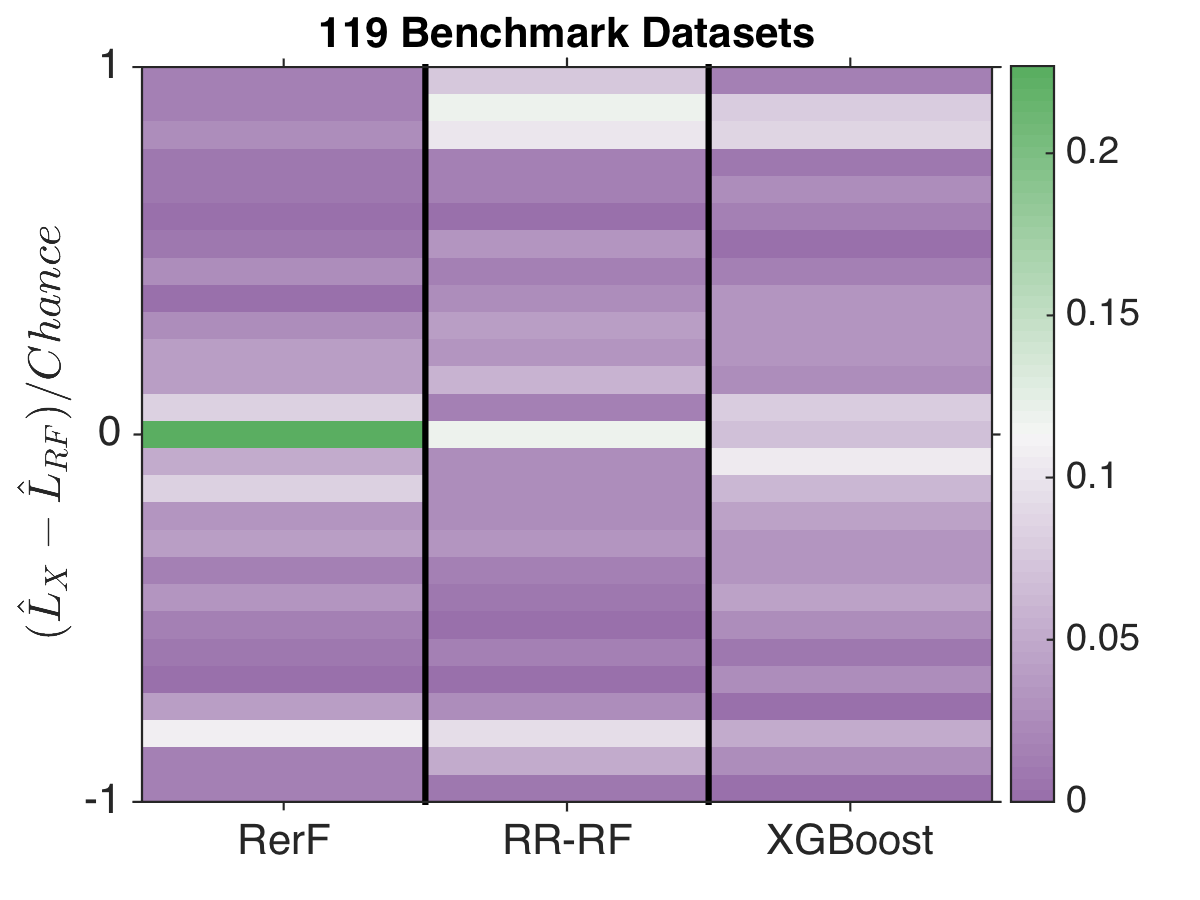
\includegraphics[height=0.4\textheight]{../../figs/rerF_benchmark.png}
\caption{
Classification performances of RF, RerF, RR-RF, and XGBoost
on 119 benchmark datasets.
}
\label{fig:RefF3}
\end{cframed}
\end{figure}

Additionally, we have made progress towards a more scalable implementation of RerF in R. The previous port of RerF to R rotated input data at the tree level instead 
of at the more desired node level.  The new port of RerF now rotates at the
node level.  The change to R will allow a fast RerF implementation by 
integrating the algorithm into FlashR.  This tool can be found \href{https://github.com/neurodata/R-RerF}{here}.


\clearpage

RerF is now working in pure R code.  The running time of this
implementation is roughly the same as the Matlab implementation for
various sizes of input.  We are re-implementing portions of the code in
both C and FlashR in an attempt to reduce the running time of the
algorithm. \\


Previously, we did not have any simulation experiments in which we know
for a fact that RF is the ``right'' thing to do. We conducted such
experiments to see how much RerF and RR-RF lose by allowing oblique
split directions. The simulated datasets were constructed as follows.
Data was sampled in $p$ dimensions over a unit hypercube centered at the
origin. Datapoints all falling into the same orthant were assigned the
same class label. Therefore, for $p$ dimensions, there are $2^p$ unique
class labels. The true decision boundary separating the classes is
purely axis-aligned. In such a case, RF is the best classifier among the
class of all ensemble tree classifiers.

\begin{figure}[!h]
\begin{cframed}
\centering
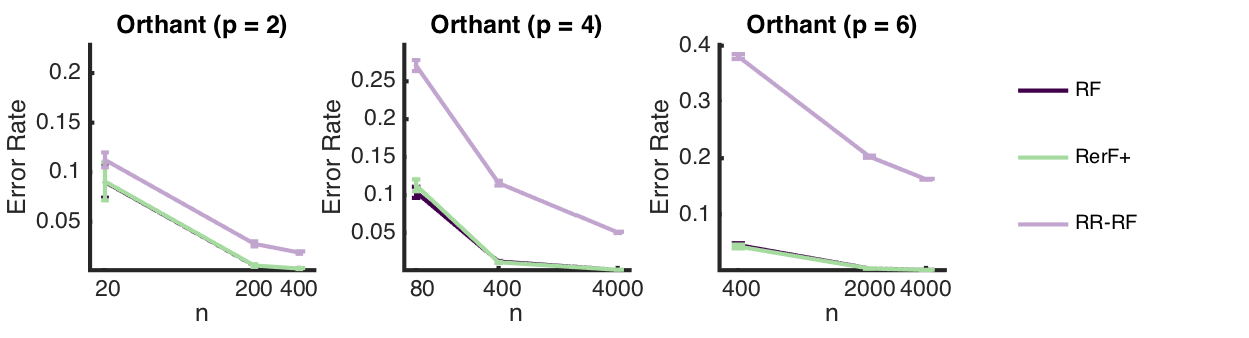
\includegraphics[width=0.85\textwidth]{../../figs/RerF_2017_02.png}
\caption{Error rate of RF, RerF, and RR-RF on the "Orthant" dataset as a
  function of $n$, the number of training samples, for three values of
  $p$. The results indicate that there is no significant difference in
  performance between RerF and RF, while RR-RF performs significantly
  worse across all settings.}
\label{fig:name}
\end{cframed}
\end{figure}


\clearpage
Most recently, we have begun investigating the theoretical behavior of RerF. Mathematical analysis of the RF and RerF procedures is difficult. Therefore, we have started with simplified procedures. The main simplifications we have made are that trees only have a depth of one (also known as decision stumps), and that each tree is trained on the full training set rather than a bootstrap sample. In the figure, we surprisingly see that RerF outperforms RF across a variety of settings (see caption for more details).

\begin{figure}[h!]
\begin{cframed}
\centering
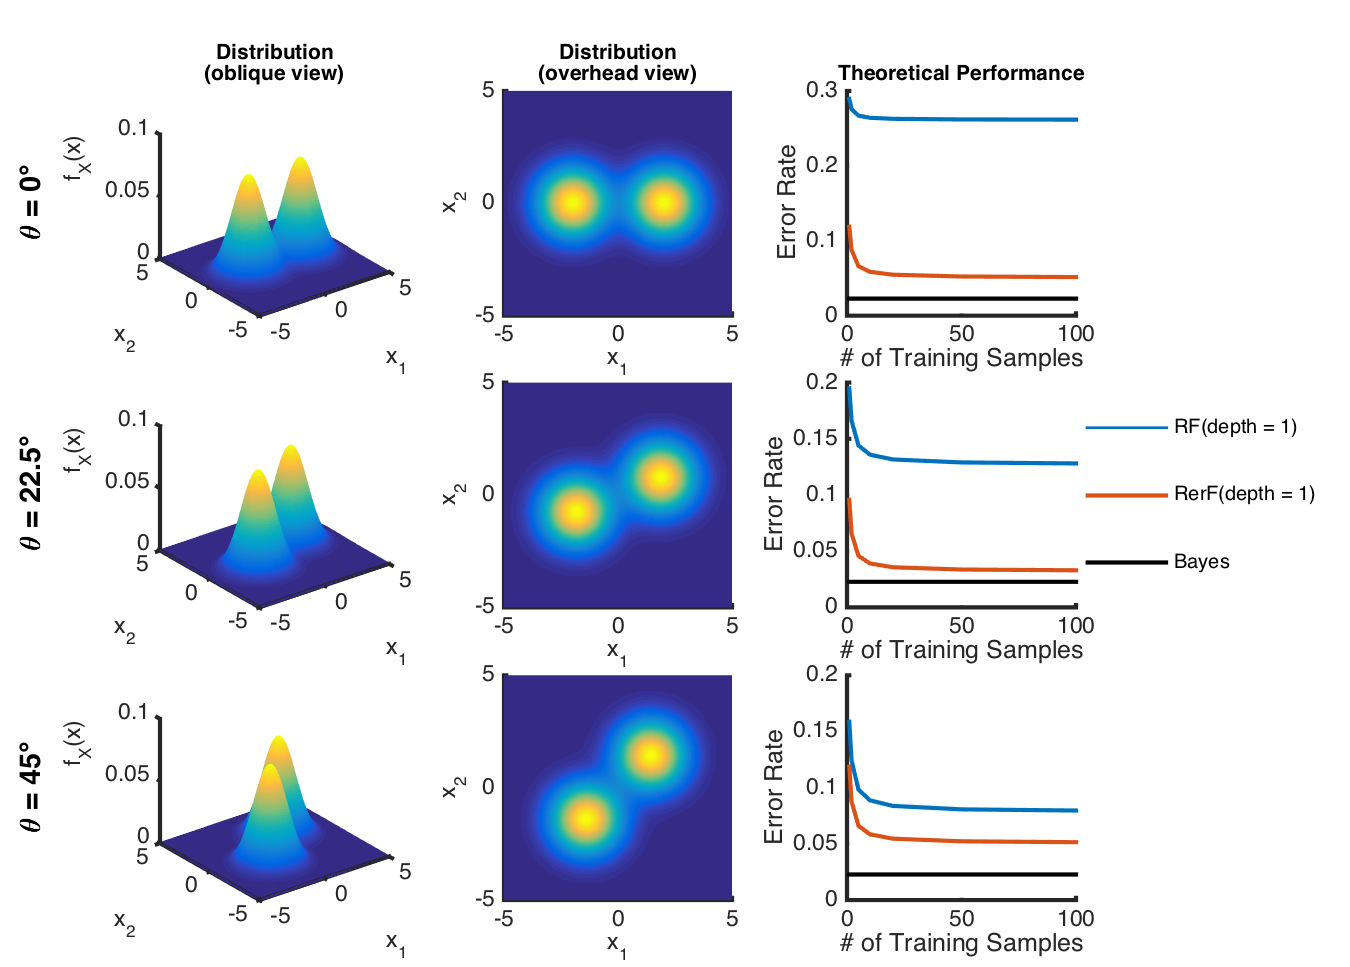
\includegraphics[height=0.4\textheight]{../../figs/RerF_2017_03.png}
\caption{
Theoretical performances of simplified RF and RerF models on a simple two-dimensional binary classification problem. In the top row, the two classes are distributed according to normal distributions having means that differ only in the first dimension and both having identity covariances. These distributions are shown in the left and middle panels. The right-most panel shows the theoretical error  rate as a function of the number of training samples for RF and RerF. The Bayes optimal error rate is also shown for reference. The middle and bottom rows are the same as the top row, except the distributions have been rotated by 22.5° and 45° respectively. In all three cases, the RerF classifier outperforms RF for all training set sizes.
}
\label{fig:RerF}
\end{cframed}
\end{figure}

The R version of RerF is now functional and is an order of magnitude faster than the Matlab implementation.  This version of RerF allows the user to specify the minimum size of a node and a parameter to tweak the rotation matrix.  Additional basic functionality is being added to this tool including bagging, out-of-bag error reporting, max tree depth, and pruning.   

\clearpage
\end{document}
